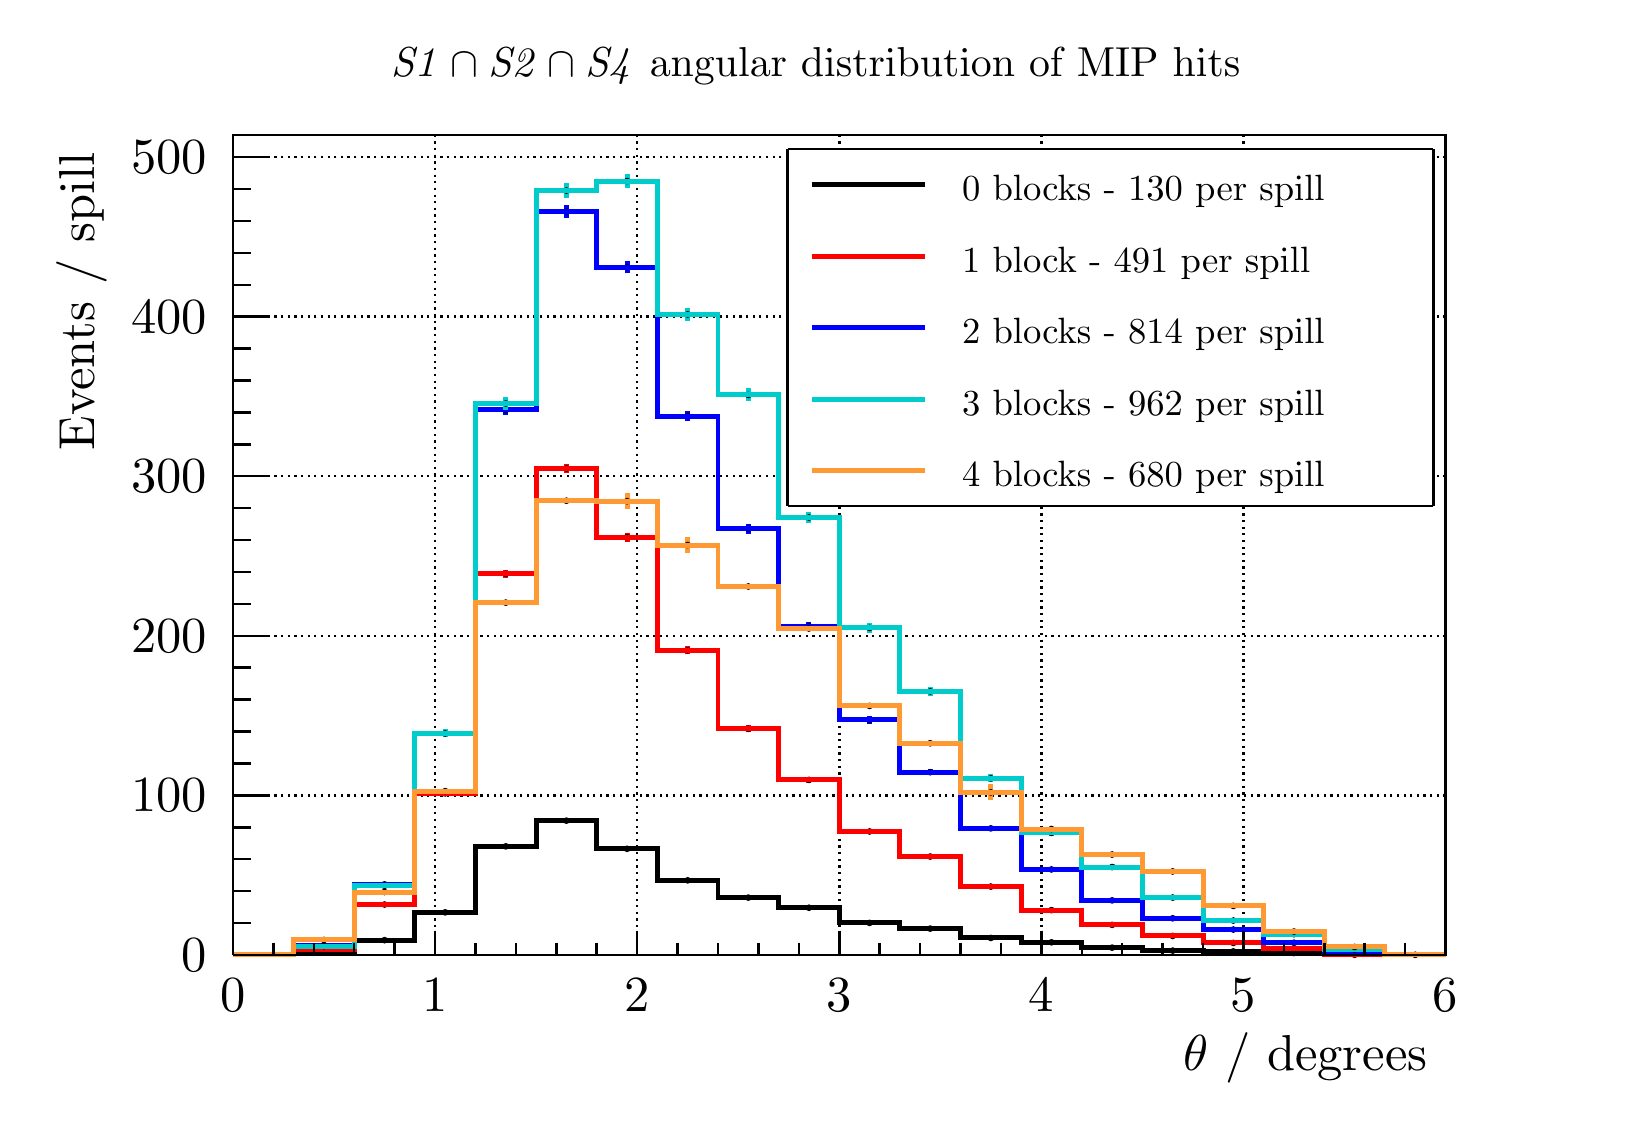
\begin{tikzpicture}
\pgfdeclareplotmark{cross} {
\pgfpathmoveto{\pgfpoint{-0.3\pgfplotmarksize}{\pgfplotmarksize}}
\pgfpathlineto{\pgfpoint{+0.3\pgfplotmarksize}{\pgfplotmarksize}}
\pgfpathlineto{\pgfpoint{+0.3\pgfplotmarksize}{0.3\pgfplotmarksize}}
\pgfpathlineto{\pgfpoint{+1\pgfplotmarksize}{0.3\pgfplotmarksize}}
\pgfpathlineto{\pgfpoint{+1\pgfplotmarksize}{-0.3\pgfplotmarksize}}
\pgfpathlineto{\pgfpoint{+0.3\pgfplotmarksize}{-0.3\pgfplotmarksize}}
\pgfpathlineto{\pgfpoint{+0.3\pgfplotmarksize}{-1.\pgfplotmarksize}}
\pgfpathlineto{\pgfpoint{-0.3\pgfplotmarksize}{-1.\pgfplotmarksize}}
\pgfpathlineto{\pgfpoint{-0.3\pgfplotmarksize}{-0.3\pgfplotmarksize}}
\pgfpathlineto{\pgfpoint{-1.\pgfplotmarksize}{-0.3\pgfplotmarksize}}
\pgfpathlineto{\pgfpoint{-1.\pgfplotmarksize}{0.3\pgfplotmarksize}}
\pgfpathlineto{\pgfpoint{-0.3\pgfplotmarksize}{0.3\pgfplotmarksize}}
\pgfpathclose
\pgfusepathqstroke
}
\pgfdeclareplotmark{cross*} {
\pgfpathmoveto{\pgfpoint{-0.3\pgfplotmarksize}{\pgfplotmarksize}}
\pgfpathlineto{\pgfpoint{+0.3\pgfplotmarksize}{\pgfplotmarksize}}
\pgfpathlineto{\pgfpoint{+0.3\pgfplotmarksize}{0.3\pgfplotmarksize}}
\pgfpathlineto{\pgfpoint{+1\pgfplotmarksize}{0.3\pgfplotmarksize}}
\pgfpathlineto{\pgfpoint{+1\pgfplotmarksize}{-0.3\pgfplotmarksize}}
\pgfpathlineto{\pgfpoint{+0.3\pgfplotmarksize}{-0.3\pgfplotmarksize}}
\pgfpathlineto{\pgfpoint{+0.3\pgfplotmarksize}{-1.\pgfplotmarksize}}
\pgfpathlineto{\pgfpoint{-0.3\pgfplotmarksize}{-1.\pgfplotmarksize}}
\pgfpathlineto{\pgfpoint{-0.3\pgfplotmarksize}{-0.3\pgfplotmarksize}}
\pgfpathlineto{\pgfpoint{-1.\pgfplotmarksize}{-0.3\pgfplotmarksize}}
\pgfpathlineto{\pgfpoint{-1.\pgfplotmarksize}{0.3\pgfplotmarksize}}
\pgfpathlineto{\pgfpoint{-0.3\pgfplotmarksize}{0.3\pgfplotmarksize}}
\pgfpathclose
\pgfusepathqfillstroke
}
\pgfdeclareplotmark{newstar} {
\pgfpathmoveto{\pgfqpoint{0pt}{\pgfplotmarksize}}
\pgfpathlineto{\pgfqpointpolar{44}{0.5\pgfplotmarksize}}
\pgfpathlineto{\pgfqpointpolar{18}{\pgfplotmarksize}}
\pgfpathlineto{\pgfqpointpolar{-20}{0.5\pgfplotmarksize}}
\pgfpathlineto{\pgfqpointpolar{-54}{\pgfplotmarksize}}
\pgfpathlineto{\pgfqpointpolar{-90}{0.5\pgfplotmarksize}}
\pgfpathlineto{\pgfqpointpolar{234}{\pgfplotmarksize}}
\pgfpathlineto{\pgfqpointpolar{198}{0.5\pgfplotmarksize}}
\pgfpathlineto{\pgfqpointpolar{162}{\pgfplotmarksize}}
\pgfpathlineto{\pgfqpointpolar{134}{0.5\pgfplotmarksize}}
\pgfpathclose
\pgfusepathqstroke
}
\pgfdeclareplotmark{newstar*} {
\pgfpathmoveto{\pgfqpoint{0pt}{\pgfplotmarksize}}
\pgfpathlineto{\pgfqpointpolar{44}{0.5\pgfplotmarksize}}
\pgfpathlineto{\pgfqpointpolar{18}{\pgfplotmarksize}}
\pgfpathlineto{\pgfqpointpolar{-20}{0.5\pgfplotmarksize}}
\pgfpathlineto{\pgfqpointpolar{-54}{\pgfplotmarksize}}
\pgfpathlineto{\pgfqpointpolar{-90}{0.5\pgfplotmarksize}}
\pgfpathlineto{\pgfqpointpolar{234}{\pgfplotmarksize}}
\pgfpathlineto{\pgfqpointpolar{198}{0.5\pgfplotmarksize}}
\pgfpathlineto{\pgfqpointpolar{162}{\pgfplotmarksize}}
\pgfpathlineto{\pgfqpointpolar{134}{0.5\pgfplotmarksize}}
\pgfpathclose
\pgfusepathqfillstroke
}
\definecolor{c}{rgb}{1,1,1};
\draw [color=c, fill=c] (0,0) rectangle (20,13.5319);
\draw [color=c, fill=c] (2.6,1.75915) rectangle (18,12.1787);
\definecolor{c}{rgb}{0,0,0};
\draw [c,line width=0.9] (2.6,1.75915) -- (2.6,12.1787) -- (18,12.1787) -- (18,1.75915) -- (2.6,1.75915);
\definecolor{c}{rgb}{1,1,1};
\draw [color=c, fill=c] (2.6,1.75915) rectangle (18,12.1787);
\definecolor{c}{rgb}{0,0,0};
\draw [c,line width=0.9] (2.6,1.75915) -- (2.6,12.1787) -- (18,12.1787) -- (18,1.75915) -- (2.6,1.75915);
\draw [c,line width=0.9] (2.6,1.75915) -- (18,1.75915);
\draw [c,dash pattern=on 0.80pt off 1.60pt ,line width=0.9] (2.6,12.1787) -- (2.6,1.75915);
\draw [c,dash pattern=on 0.80pt off 1.60pt ,line width=0.9] (5.16667,12.1787) -- (5.16667,1.75915);
\draw [c,dash pattern=on 0.80pt off 1.60pt ,line width=0.9] (7.73333,12.1787) -- (7.73333,1.75915);
\draw [c,dash pattern=on 0.80pt off 1.60pt ,line width=0.9] (10.3,12.1787) -- (10.3,1.75915);
\draw [c,dash pattern=on 0.80pt off 1.60pt ,line width=0.9] (12.8667,12.1787) -- (12.8667,1.75915);
\draw [c,dash pattern=on 0.80pt off 1.60pt ,line width=0.9] (15.4333,12.1787) -- (15.4333,1.75915);
\draw [c,dash pattern=on 0.80pt off 1.60pt ,line width=0.9] (18,12.1787) -- (18,1.75915);
\draw [c,line width=0.9] (2.6,1.75915) -- (2.6,12.1787);
\draw [c,dash pattern=on 0.80pt off 1.60pt ,line width=0.9] (18,1.76314) -- (2.6,1.76314);
\draw [c,dash pattern=on 0.80pt off 1.60pt ,line width=0.9] (18,3.78938) -- (2.6,3.78938);
\draw [c,dash pattern=on 0.80pt off 1.60pt ,line width=0.9] (18,5.81563) -- (2.6,5.81563);
\draw [c,dash pattern=on 0.80pt off 1.60pt ,line width=0.9] (18,7.84188) -- (2.6,7.84188);
\draw [c,dash pattern=on 0.80pt off 1.60pt ,line width=0.9] (18,9.86813) -- (2.6,9.86813);
\draw [c,dash pattern=on 0.80pt off 1.60pt ,line width=0.9] (18,11.8944) -- (2.6,11.8944);
\draw [c,dash pattern=on 0.80pt off 1.60pt ,line width=0.9] (18,1.76314) -- (2.6,1.76314);
\draw [c,dash pattern=on 0.80pt off 1.60pt ,line width=0.9] (18,11.8944) -- (2.6,11.8944);
\definecolor{c}{rgb}{0,0,0.6};
\draw [c,line width=0.9] (2.6,1.76314) -- (3.37,1.76314) -- (3.37,1.76314) -- (4.14,1.76314) -- (4.14,1.76314) -- (4.91,1.76314) -- (4.91,1.76314) -- (5.68,1.76314) -- (5.68,1.76314) -- (6.45,1.76314) -- (6.45,1.76314) -- (7.22,1.76314) --
 (7.22,1.76314) -- (7.99,1.76314) -- (7.99,1.76314) -- (8.76,1.76314) -- (8.76,1.76314) -- (9.53,1.76314) -- (9.53,1.76314) -- (10.3,1.76314) -- (10.3,1.76314) -- (11.07,1.76314) -- (11.07,1.76314) -- (11.84,1.76314) -- (11.84,1.76314) --
 (12.61,1.76314) -- (12.61,1.76314) -- (13.38,1.76314) -- (13.38,1.76314) -- (14.15,1.76314) -- (14.15,1.76314) -- (14.92,1.76314) -- (14.92,1.76314) -- (15.69,1.76314) -- (15.69,1.76314) -- (16.46,1.76314) -- (16.46,1.76314) -- (17.23,1.76314) --
 (17.23,1.76314) -- (18,1.76314);
\definecolor{c}{rgb}{0,0,0};
\draw [c,line width=0.9] (2.6,1.75915) -- (18,1.75915);
\draw [c,line width=0.9] (2.6,2.07174) -- (2.6,1.75915);
\draw [c,line width=0.9] (3.11333,1.91544) -- (3.11333,1.75915);
\draw [c,line width=0.9] (3.62667,1.91544) -- (3.62667,1.75915);
\draw [c,line width=0.9] (4.14,1.91544) -- (4.14,1.75915);
\draw [c,line width=0.9] (4.65333,1.91544) -- (4.65333,1.75915);
\draw [c,line width=0.9] (5.16667,2.07174) -- (5.16667,1.75915);
\draw [c,line width=0.9] (5.68,1.91544) -- (5.68,1.75915);
\draw [c,line width=0.9] (6.19333,1.91544) -- (6.19333,1.75915);
\draw [c,line width=0.9] (6.70667,1.91544) -- (6.70667,1.75915);
\draw [c,line width=0.9] (7.22,1.91544) -- (7.22,1.75915);
\draw [c,line width=0.9] (7.73333,2.07174) -- (7.73333,1.75915);
\draw [c,line width=0.9] (8.24667,1.91544) -- (8.24667,1.75915);
\draw [c,line width=0.9] (8.76,1.91544) -- (8.76,1.75915);
\draw [c,line width=0.9] (9.27333,1.91544) -- (9.27333,1.75915);
\draw [c,line width=0.9] (9.78667,1.91544) -- (9.78667,1.75915);
\draw [c,line width=0.9] (10.3,2.07174) -- (10.3,1.75915);
\draw [c,line width=0.9] (10.8133,1.91544) -- (10.8133,1.75915);
\draw [c,line width=0.9] (11.3267,1.91544) -- (11.3267,1.75915);
\draw [c,line width=0.9] (11.84,1.91544) -- (11.84,1.75915);
\draw [c,line width=0.9] (12.3533,1.91544) -- (12.3533,1.75915);
\draw [c,line width=0.9] (12.8667,2.07174) -- (12.8667,1.75915);
\draw [c,line width=0.9] (13.38,1.91544) -- (13.38,1.75915);
\draw [c,line width=0.9] (13.8933,1.91544) -- (13.8933,1.75915);
\draw [c,line width=0.9] (14.4067,1.91544) -- (14.4067,1.75915);
\draw [c,line width=0.9] (14.92,1.91544) -- (14.92,1.75915);
\draw [c,line width=0.9] (15.4333,2.07174) -- (15.4333,1.75915);
\draw [c,line width=0.9] (15.9467,1.91544) -- (15.9467,1.75915);
\draw [c,line width=0.9] (16.46,1.91544) -- (16.46,1.75915);
\draw [c,line width=0.9] (16.9733,1.91544) -- (16.9733,1.75915);
\draw [c,line width=0.9] (17.4867,1.91544) -- (17.4867,1.75915);
\draw [c,line width=0.9] (18,2.07174) -- (18,1.75915);
\draw [anchor=base] (2.6,1.04196) node[scale=1.82718, color=c, rotate=0]{0};
\draw [anchor=base] (5.16667,1.04196) node[scale=1.82718, color=c, rotate=0]{1};
\draw [anchor=base] (7.73333,1.04196) node[scale=1.82718, color=c, rotate=0]{2};
\draw [anchor=base] (10.3,1.04196) node[scale=1.82718, color=c, rotate=0]{3};
\draw [anchor=base] (12.8667,1.04196) node[scale=1.82718, color=c, rotate=0]{4};
\draw [anchor=base] (15.4333,1.04196) node[scale=1.82718, color=c, rotate=0]{5};
\draw [anchor=base] (18,1.04196) node[scale=1.82718, color=c, rotate=0]{6};
\draw [anchor= east] (18,0.460085) node[scale=1.82718, color=c, rotate=0]{$\theta$ / degrees};
\draw [c,line width=0.9] (2.6,1.75915) -- (2.6,12.1787);
\draw [c,line width=0.9] (3.062,1.76314) -- (2.6,1.76314);
\draw [c,line width=0.9] (2.831,2.16839) -- (2.6,2.16839);
\draw [c,line width=0.9] (2.831,2.57364) -- (2.6,2.57364);
\draw [c,line width=0.9] (2.831,2.97889) -- (2.6,2.97889);
\draw [c,line width=0.9] (2.831,3.38414) -- (2.6,3.38414);
\draw [c,line width=0.9] (3.062,3.78938) -- (2.6,3.78938);
\draw [c,line width=0.9] (2.831,4.19463) -- (2.6,4.19463);
\draw [c,line width=0.9] (2.831,4.59988) -- (2.6,4.59988);
\draw [c,line width=0.9] (2.831,5.00513) -- (2.6,5.00513);
\draw [c,line width=0.9] (2.831,5.41038) -- (2.6,5.41038);
\draw [c,line width=0.9] (3.062,5.81563) -- (2.6,5.81563);
\draw [c,line width=0.9] (2.831,6.22088) -- (2.6,6.22088);
\draw [c,line width=0.9] (2.831,6.62613) -- (2.6,6.62613);
\draw [c,line width=0.9] (2.831,7.03138) -- (2.6,7.03138);
\draw [c,line width=0.9] (2.831,7.43663) -- (2.6,7.43663);
\draw [c,line width=0.9] (3.062,7.84188) -- (2.6,7.84188);
\draw [c,line width=0.9] (2.831,8.24713) -- (2.6,8.24713);
\draw [c,line width=0.9] (2.831,8.65238) -- (2.6,8.65238);
\draw [c,line width=0.9] (2.831,9.05763) -- (2.6,9.05763);
\draw [c,line width=0.9] (2.831,9.46288) -- (2.6,9.46288);
\draw [c,line width=0.9] (3.062,9.86813) -- (2.6,9.86813);
\draw [c,line width=0.9] (2.831,10.2734) -- (2.6,10.2734);
\draw [c,line width=0.9] (2.831,10.6786) -- (2.6,10.6786);
\draw [c,line width=0.9] (2.831,11.0839) -- (2.6,11.0839);
\draw [c,line width=0.9] (2.831,11.4891) -- (2.6,11.4891);
\draw [c,line width=0.9] (3.062,11.8944) -- (2.6,11.8944);
\draw [c,line width=0.9] (3.062,1.76314) -- (2.6,1.76314);
\draw [c,line width=0.9] (3.062,11.8944) -- (2.6,11.8944);
\draw [anchor= east] (2.5,1.76314) node[scale=1.82718, color=c, rotate=0]{0};
\draw [anchor= east] (2.5,3.78938) node[scale=1.82718, color=c, rotate=0]{100};
\draw [anchor= east] (2.5,5.81563) node[scale=1.82718, color=c, rotate=0]{200};
\draw [anchor= east] (2.5,7.84188) node[scale=1.82718, color=c, rotate=0]{300};
\draw [anchor= east] (2.5,9.86813) node[scale=1.82718, color=c, rotate=0]{400};
\draw [anchor= east] (2.5,11.8944) node[scale=1.82718, color=c, rotate=0]{500};
\draw [anchor= east] (0.68,12.1787) node[scale=1.82718, color=c, rotate=90]{ Events / spill};
\draw [c,line width=1.8] (3.755,1.79593) -- (3.755,1.80261);
\draw [c,line width=1.8] (3.755,1.80261) -- (3.755,1.80929);
\foreach \P in {(3.755,1.80261)}{\draw[mark options={color=c,fill=c},mark size=2.402402pt,mark=*,mark size=1pt] plot coordinates {\P};}
\draw [c,line width=1.8] (4.525,1.93666) -- (4.525,1.95047);
\draw [c,line width=1.8] (4.525,1.95047) -- (4.525,1.96428);
\foreach \P in {(4.525,1.95047)}{\draw[mark options={color=c,fill=c},mark size=2.402402pt,mark=*,mark size=1pt] plot coordinates {\P};}
\draw [c,line width=1.8] (5.295,2.28176) -- (5.295,2.30352);
\draw [c,line width=1.8] (5.295,2.30352) -- (5.295,2.32527);
\foreach \P in {(5.295,2.30352)}{\draw[mark options={color=c,fill=c},mark size=2.402402pt,mark=*,mark size=1pt] plot coordinates {\P};}
\draw [c,line width=1.8] (6.065,3.10901) -- (6.065,3.14165);
\draw [c,line width=1.8] (6.065,3.14165) -- (6.065,3.17429);
\foreach \P in {(6.065,3.14165)}{\draw[mark options={color=c,fill=c},mark size=2.402402pt,mark=*,mark size=1pt] plot coordinates {\P};}
\draw [c,line width=1.8] (6.835,3.43299) -- (6.835,3.46832);
\draw [c,line width=1.8] (6.835,3.46832) -- (6.835,3.50364);
\foreach \P in {(6.835,3.46832)}{\draw[mark options={color=c,fill=c},mark size=2.402402pt,mark=*,mark size=1pt] plot coordinates {\P};}
\draw [c,line width=1.8] (7.605,3.07863) -- (7.605,3.11047);
\draw [c,line width=1.8] (7.605,3.11047) -- (7.605,3.14232);
\foreach \P in {(7.605,3.11047)}{\draw[mark options={color=c,fill=c},mark size=2.402402pt,mark=*,mark size=1pt] plot coordinates {\P};}
\draw [c,line width=1.8] (8.375,2.68238) -- (8.375,2.71);
\draw [c,line width=1.8] (8.375,2.71) -- (8.375,2.73763);
\foreach \P in {(8.375,2.71)}{\draw[mark options={color=c,fill=c},mark size=2.402402pt,mark=*,mark size=1pt] plot coordinates {\P};}
\draw [c,line width=1.8] (9.145,2.46596) -- (9.145,2.4906);
\draw [c,line width=1.8] (9.145,2.4906) -- (9.145,2.51525);
\foreach \P in {(9.145,2.4906)}{\draw[mark options={color=c,fill=c},mark size=2.402402pt,mark=*,mark size=1pt] plot coordinates {\P};}
\draw [c,line width=1.8] (9.915,2.33946) -- (9.915,2.36213);
\draw [c,line width=1.8] (9.915,2.36213) -- (9.915,2.3848);
\foreach \P in {(9.915,2.36213)}{\draw[mark options={color=c,fill=c},mark size=2.402402pt,mark=*,mark size=1pt] plot coordinates {\P};}
\draw [c,line width=1.8] (10.685,2.15064) -- (10.685,2.16968);
\draw [c,line width=1.8] (10.685,2.16968) -- (10.685,2.18872);
\foreach \P in {(10.685,2.16968)}{\draw[mark options={color=c,fill=c},mark size=2.402402pt,mark=*,mark size=1pt] plot coordinates {\P};}
\draw [c,line width=1.8] (11.455,2.0798) -- (11.455,2.09712);
\draw [c,line width=1.8] (11.455,2.09712) -- (11.455,2.11443);
\foreach \P in {(11.455,2.09712)}{\draw[mark options={color=c,fill=c},mark size=2.402402pt,mark=*,mark size=1pt] plot coordinates {\P};}
\draw [c,line width=1.8] (12.225,1.96416) -- (12.225,1.97816);
\draw [c,line width=1.8] (12.225,1.97816) -- (12.225,1.99215);
\foreach \P in {(12.225,1.97816)}{\draw[mark options={color=c,fill=c},mark size=2.402402pt,mark=*,mark size=1pt] plot coordinates {\P};}
\draw [c,line width=1.8] (12.995,1.91031) -- (12.995,1.9229);
\draw [c,line width=1.8] (12.995,1.9229) -- (12.995,1.9355);
\foreach \P in {(12.995,1.9229)}{\draw[mark options={color=c,fill=c},mark size=2.402402pt,mark=*,mark size=1pt] plot coordinates {\P};}
\draw [c,line width=1.8] (13.765,1.84567) -- (13.765,1.85541);
\draw [c,line width=1.8] (13.765,1.85541) -- (13.765,1.86516);
\foreach \P in {(13.765,1.85541)}{\draw[mark options={color=c,fill=c},mark size=2.402402pt,mark=*,mark size=1pt] plot coordinates {\P};}
\draw [c,line width=1.8] (14.535,1.80977) -- (14.535,1.81763);
\draw [c,line width=1.8] (14.535,1.81763) -- (14.535,1.82549);
\foreach \P in {(14.535,1.81763)}{\draw[mark options={color=c,fill=c},mark size=2.402402pt,mark=*,mark size=1pt] plot coordinates {\P};}
\draw [c,line width=1.8] (15.305,1.80006) -- (15.305,1.80753);
\draw [c,line width=1.8] (15.305,1.80753) -- (15.305,1.81501);
\foreach \P in {(15.305,1.80753)}{\draw[mark options={color=c,fill=c},mark size=2.402402pt,mark=*,mark size=1pt] plot coordinates {\P};}
\draw [c,line width=1.8] (16.075,1.78173) -- (16.075,1.78745);
\draw [c,line width=1.8] (16.075,1.78745) -- (16.075,1.79316);
\foreach \P in {(16.075,1.78745)}{\draw[mark options={color=c,fill=c},mark size=2.402402pt,mark=*,mark size=1pt] plot coordinates {\P};}
\draw [c,line width=1.8] (16.845,1.76211) -- (16.845,1.76529);
\draw [c,line width=1.8] (16.845,1.76529) -- (16.845,1.76847);
\foreach \P in {(16.845,1.76529)}{\draw[mark options={color=c,fill=c},mark size=2.402402pt,mark=*,mark size=1pt] plot coordinates {\P};}
\draw [c,line width=1.8] (2.6,1.76314) -- (3.37,1.76314) -- (3.37,1.80261) -- (4.14,1.80261) -- (4.14,1.95047) -- (4.91,1.95047) -- (4.91,2.30352) -- (5.68,2.30352) -- (5.68,3.14165) -- (6.45,3.14165) -- (6.45,3.46832) -- (7.22,3.46832) --
 (7.22,3.11047) -- (7.99,3.11047) -- (7.99,2.71) -- (8.76,2.71) -- (8.76,2.4906) -- (9.53,2.4906) -- (9.53,2.36213) -- (10.3,2.36213) -- (10.3,2.16968) -- (11.07,2.16968) -- (11.07,2.09712) -- (11.84,2.09712) -- (11.84,1.97816) -- (12.61,1.97816) --
 (12.61,1.9229) -- (13.38,1.9229) -- (13.38,1.85541) -- (14.15,1.85541) -- (14.15,1.81763) -- (14.92,1.81763) -- (14.92,1.80753) -- (15.69,1.80753) -- (15.69,1.78745) -- (16.46,1.78745) -- (16.46,1.76529) -- (17.23,1.76529) -- (17.23,1.76314) --
 (18,1.76314);
\definecolor{c}{rgb}{1,0,0};
\draw [c,line width=1.8] (3.755,1.82556) -- (3.755,1.83317);
\draw [c,line width=1.8] (3.755,1.83317) -- (3.755,1.84077);
\definecolor{c}{rgb}{0,0,0};
\foreach \P in {(3.755,1.83317)}{\draw[mark options={color=c,fill=c},mark size=2.402402pt,mark=*,mark size=1pt] plot coordinates {\P};}
\definecolor{c}{rgb}{1,0,0};
\draw [c,line width=1.8] (4.525,2.38144) -- (4.525,2.40275);
\draw [c,line width=1.8] (4.525,2.40275) -- (4.525,2.42406);
\definecolor{c}{rgb}{0,0,0};
\foreach \P in {(4.525,2.40275)}{\draw[mark options={color=c,fill=c},mark size=2.402402pt,mark=*,mark size=1pt] plot coordinates {\P};}
\definecolor{c}{rgb}{1,0,0};
\draw [c,line width=1.8] (5.295,3.77778) -- (5.295,3.81419);
\draw [c,line width=1.8] (5.295,3.81419) -- (5.295,3.85061);
\definecolor{c}{rgb}{0,0,0};
\foreach \P in {(5.295,3.81419)}{\draw[mark options={color=c,fill=c},mark size=2.402402pt,mark=*,mark size=1pt] plot coordinates {\P};}
\definecolor{c}{rgb}{1,0,0};
\draw [c,line width=1.8] (6.065,6.54763) -- (6.065,6.60255);
\draw [c,line width=1.8] (6.065,6.60255) -- (6.065,6.65746);
\definecolor{c}{rgb}{0,0,0};
\foreach \P in {(6.065,6.60255)}{\draw[mark options={color=c,fill=c},mark size=2.402402pt,mark=*,mark size=1pt] plot coordinates {\P};}
\definecolor{c}{rgb}{1,0,0};
\draw [c,line width=1.8] (6.835,7.87871) -- (6.835,7.94038);
\draw [c,line width=1.8] (6.835,7.94038) -- (6.835,8.00206);
\definecolor{c}{rgb}{0,0,0};
\foreach \P in {(6.835,7.94038)}{\draw[mark options={color=c,fill=c},mark size=2.402402pt,mark=*,mark size=1pt] plot coordinates {\P};}
\definecolor{c}{rgb}{1,0,0};
\draw [c,line width=1.8] (7.605,7.01081) -- (7.605,7.06893);
\draw [c,line width=1.8] (7.605,7.06893) -- (7.605,7.12705);
\definecolor{c}{rgb}{0,0,0};
\foreach \P in {(7.605,7.06893)}{\draw[mark options={color=c,fill=c},mark size=2.402402pt,mark=*,mark size=1pt] plot coordinates {\P};}
\definecolor{c}{rgb}{1,0,0};
\draw [c,line width=1.8] (8.375,5.57969) -- (8.375,5.62986);
\draw [c,line width=1.8] (8.375,5.62986) -- (8.375,5.68002);
\definecolor{c}{rgb}{0,0,0};
\foreach \P in {(8.375,5.62986)}{\draw[mark options={color=c,fill=c},mark size=2.402402pt,mark=*,mark size=1pt] plot coordinates {\P};}
\definecolor{c}{rgb}{1,0,0};
\draw [c,line width=1.8] (9.145,4.59003) -- (9.145,4.63431);
\draw [c,line width=1.8] (9.145,4.63431) -- (9.145,4.67859);
\definecolor{c}{rgb}{0,0,0};
\foreach \P in {(9.145,4.63431)}{\draw[mark options={color=c,fill=c},mark size=2.402402pt,mark=*,mark size=1pt] plot coordinates {\P};}
\definecolor{c}{rgb}{1,0,0};
\draw [c,line width=1.8] (9.915,3.94666) -- (9.915,3.98587);
\draw [c,line width=1.8] (9.915,3.98587) -- (9.915,4.02509);
\definecolor{c}{rgb}{0,0,0};
\foreach \P in {(9.915,3.98587)}{\draw[mark options={color=c,fill=c},mark size=2.402402pt,mark=*,mark size=1pt] plot coordinates {\P};}
\definecolor{c}{rgb}{1,0,0};
\draw [c,line width=1.8] (10.685,3.29695) -- (10.685,3.33072);
\draw [c,line width=1.8] (10.685,3.33072) -- (10.685,3.36448);
\definecolor{c}{rgb}{0,0,0};
\foreach \P in {(10.685,3.33072)}{\draw[mark options={color=c,fill=c},mark size=2.402402pt,mark=*,mark size=1pt] plot coordinates {\P};}
\definecolor{c}{rgb}{1,0,0};
\draw [c,line width=1.8] (11.455,2.98195) -- (11.455,3.01238);
\draw [c,line width=1.8] (11.455,3.01238) -- (11.455,3.04281);
\definecolor{c}{rgb}{0,0,0};
\foreach \P in {(11.455,3.01238)}{\draw[mark options={color=c,fill=c},mark size=2.402402pt,mark=*,mark size=1pt] plot coordinates {\P};}
\definecolor{c}{rgb}{1,0,0};
\draw [c,line width=1.8] (12.225,2.60494) -- (12.225,2.63083);
\draw [c,line width=1.8] (12.225,2.63083) -- (12.225,2.65672);
\definecolor{c}{rgb}{0,0,0};
\foreach \P in {(12.225,2.63083)}{\draw[mark options={color=c,fill=c},mark size=2.402402pt,mark=*,mark size=1pt] plot coordinates {\P};}
\definecolor{c}{rgb}{1,0,0};
\draw [c,line width=1.8] (12.995,2.31005) -- (12.995,2.33181);
\draw [c,line width=1.8] (12.995,2.33181) -- (12.995,2.35357);
\definecolor{c}{rgb}{0,0,0};
\foreach \P in {(12.995,2.33181)}{\draw[mark options={color=c,fill=c},mark size=2.402402pt,mark=*,mark size=1pt] plot coordinates {\P};}
\definecolor{c}{rgb}{1,0,0};
\draw [c,line width=1.8] (13.765,2.1258) -- (13.765,2.14441);
\draw [c,line width=1.8] (13.765,2.14441) -- (13.765,2.16303);
\definecolor{c}{rgb}{0,0,0};
\foreach \P in {(13.765,2.14441)}{\draw[mark options={color=c,fill=c},mark size=2.402402pt,mark=*,mark size=1pt] plot coordinates {\P};}
\definecolor{c}{rgb}{1,0,0};
\draw [c,line width=1.8] (14.535,1.98933) -- (14.535,2.00437);
\draw [c,line width=1.8] (14.535,2.00437) -- (14.535,2.0194);
\definecolor{c}{rgb}{0,0,0};
\foreach \P in {(14.535,2.00437)}{\draw[mark options={color=c,fill=c},mark size=2.402402pt,mark=*,mark size=1pt] plot coordinates {\P};}
\definecolor{c}{rgb}{1,0,0};
\draw [c,line width=1.8] (15.305,1.90262) -- (15.305,1.91538);
\draw [c,line width=1.8] (15.305,1.91538) -- (15.305,1.92813);
\definecolor{c}{rgb}{0,0,0};
\foreach \P in {(15.305,1.91538)}{\draw[mark options={color=c,fill=c},mark size=2.402402pt,mark=*,mark size=1pt] plot coordinates {\P};}
\definecolor{c}{rgb}{1,0,0};
\draw [c,line width=1.8] (16.075,1.83617) -- (16.075,1.84692);
\draw [c,line width=1.8] (16.075,1.84692) -- (16.075,1.85767);
\definecolor{c}{rgb}{0,0,0};
\foreach \P in {(16.075,1.84692)}{\draw[mark options={color=c,fill=c},mark size=2.402402pt,mark=*,mark size=1pt] plot coordinates {\P};}
\definecolor{c}{rgb}{1,0,0};
\draw [c,line width=1.8] (16.845,1.76562) -- (16.845,1.7714);
\draw [c,line width=1.8] (16.845,1.7714) -- (16.845,1.77718);
\definecolor{c}{rgb}{0,0,0};
\foreach \P in {(16.845,1.7714)}{\draw[mark options={color=c,fill=c},mark size=2.402402pt,mark=*,mark size=1pt] plot coordinates {\P};}
\definecolor{c}{rgb}{1,0,0};
\draw [c,line width=1.8] (2.6,1.76314) -- (3.37,1.76314) -- (3.37,1.83317) -- (4.14,1.83317) -- (4.14,2.40275) -- (4.91,2.40275) -- (4.91,3.81419) -- (5.68,3.81419) -- (5.68,6.60255) -- (6.45,6.60255) -- (6.45,7.94038) -- (7.22,7.94038) --
 (7.22,7.06893) -- (7.99,7.06893) -- (7.99,5.62986) -- (8.76,5.62986) -- (8.76,4.63431) -- (9.53,4.63431) -- (9.53,3.98587) -- (10.3,3.98587) -- (10.3,3.33072) -- (11.07,3.33072) -- (11.07,3.01238) -- (11.84,3.01238) -- (11.84,2.63083) --
 (12.61,2.63083) -- (12.61,2.33181) -- (13.38,2.33181) -- (13.38,2.14441) -- (14.15,2.14441) -- (14.15,2.00437) -- (14.92,2.00437) -- (14.92,1.91538) -- (15.69,1.91538) -- (15.69,1.84692) -- (16.46,1.84692) -- (16.46,1.7714) -- (17.23,1.7714) --
 (17.23,1.76314) -- (18,1.76314);
\definecolor{c}{rgb}{0,0,1};
\draw [c,line width=1.8] (3.755,1.86671) -- (3.755,1.87683);
\draw [c,line width=1.8] (3.755,1.87683) -- (3.755,1.88695);
\definecolor{c}{rgb}{0,0,0};
\foreach \P in {(3.755,1.87683)}{\draw[mark options={color=c,fill=c},mark size=2.402402pt,mark=*,mark size=1pt] plot coordinates {\P};}
\definecolor{c}{rgb}{0,0,1};
\draw [c,line width=1.8] (4.525,2.6329) -- (4.525,2.65891);
\draw [c,line width=1.8] (4.525,2.65891) -- (4.525,2.68492);
\definecolor{c}{rgb}{0,0,0};
\foreach \P in {(4.525,2.65891)}{\draw[mark options={color=c,fill=c},mark size=2.402402pt,mark=*,mark size=1pt] plot coordinates {\P};}
\definecolor{c}{rgb}{0,0,1};
\draw [c,line width=1.8] (5.295,4.53328) -- (5.295,4.57729);
\draw [c,line width=1.8] (5.295,4.57729) -- (5.295,4.62129);
\definecolor{c}{rgb}{0,0,0};
\foreach \P in {(5.295,4.57729)}{\draw[mark options={color=c,fill=c},mark size=2.402402pt,mark=*,mark size=1pt] plot coordinates {\P};}
\definecolor{c}{rgb}{0,0,1};
\draw [c,line width=1.8] (6.065,8.61669) -- (6.065,8.68364);
\draw [c,line width=1.8] (6.065,8.68364) -- (6.065,8.75058);
\definecolor{c}{rgb}{0,0,0};
\foreach \P in {(6.065,8.68364)}{\draw[mark options={color=c,fill=c},mark size=2.402402pt,mark=*,mark size=1pt] plot coordinates {\P};}
\definecolor{c}{rgb}{0,0,1};
\draw [c,line width=1.8] (6.835,11.1277) -- (6.835,11.2047);
\draw [c,line width=1.8] (6.835,11.2047) -- (6.835,11.2818);
\definecolor{c}{rgb}{0,0,0};
\foreach \P in {(6.835,11.2047)}{\draw[mark options={color=c,fill=c},mark size=2.402402pt,mark=*,mark size=1pt] plot coordinates {\P};}
\definecolor{c}{rgb}{0,0,1};
\draw [c,line width=1.8] (7.605,10.421) -- (7.605,10.4955);
\draw [c,line width=1.8] (7.605,10.4955) -- (7.605,10.5699);
\definecolor{c}{rgb}{0,0,0};
\foreach \P in {(7.605,10.4955)}{\draw[mark options={color=c,fill=c},mark size=2.402402pt,mark=*,mark size=1pt] plot coordinates {\P};}
\definecolor{c}{rgb}{0,0,1};
\draw [c,line width=1.8] (8.375,8.53976) -- (8.375,8.60693);
\draw [c,line width=1.8] (8.375,8.60693) -- (8.375,8.6741);
\definecolor{c}{rgb}{0,0,0};
\foreach \P in {(8.375,8.60693)}{\draw[mark options={color=c,fill=c},mark size=2.402402pt,mark=*,mark size=1pt] plot coordinates {\P};}
\definecolor{c}{rgb}{0,0,1};
\draw [c,line width=1.8] (9.145,7.11426) -- (9.145,7.17532);
\draw [c,line width=1.8] (9.145,7.17532) -- (9.145,7.23639);
\definecolor{c}{rgb}{0,0,0};
\foreach \P in {(9.145,7.17532)}{\draw[mark options={color=c,fill=c},mark size=2.402402pt,mark=*,mark size=1pt] plot coordinates {\P};}
\definecolor{c}{rgb}{0,0,1};
\draw [c,line width=1.8] (9.915,5.88203) -- (9.915,5.93612);
\draw [c,line width=1.8] (9.915,5.93612) -- (9.915,5.9902);
\definecolor{c}{rgb}{0,0,0};
\foreach \P in {(9.915,5.93612)}{\draw[mark options={color=c,fill=c},mark size=2.402402pt,mark=*,mark size=1pt] plot coordinates {\P};}
\definecolor{c}{rgb}{0,0,1};
\draw [c,line width=1.8] (10.685,4.70003) -- (10.685,4.74684);
\draw [c,line width=1.8] (10.685,4.74684) -- (10.685,4.79366);
\definecolor{c}{rgb}{0,0,0};
\foreach \P in {(10.685,4.74684)}{\draw[mark options={color=c,fill=c},mark size=2.402402pt,mark=*,mark size=1pt] plot coordinates {\P};}
\definecolor{c}{rgb}{0,0,1};
\draw [c,line width=1.8] (11.455,4.0418) -- (11.455,4.0834);
\draw [c,line width=1.8] (11.455,4.0834) -- (11.455,4.125);
\definecolor{c}{rgb}{0,0,0};
\foreach \P in {(11.455,4.0834)}{\draw[mark options={color=c,fill=c},mark size=2.402402pt,mark=*,mark size=1pt] plot coordinates {\P};}
\definecolor{c}{rgb}{0,0,1};
\draw [c,line width=1.8] (12.225,3.33469) -- (12.225,3.36999);
\draw [c,line width=1.8] (12.225,3.36999) -- (12.225,3.40529);
\definecolor{c}{rgb}{0,0,0};
\foreach \P in {(12.225,3.36999)}{\draw[mark options={color=c,fill=c},mark size=2.402402pt,mark=*,mark size=1pt] plot coordinates {\P};}
\definecolor{c}{rgb}{0,0,1};
\draw [c,line width=1.8] (12.995,2.81804) -- (12.995,2.84839);
\draw [c,line width=1.8] (12.995,2.84839) -- (12.995,2.87875);
\definecolor{c}{rgb}{0,0,0};
\foreach \P in {(12.995,2.84839)}{\draw[mark options={color=c,fill=c},mark size=2.402402pt,mark=*,mark size=1pt] plot coordinates {\P};}
\definecolor{c}{rgb}{0,0,1};
\draw [c,line width=1.8] (13.765,2.43047) -- (13.765,2.45556);
\draw [c,line width=1.8] (13.765,2.45556) -- (13.765,2.48065);
\definecolor{c}{rgb}{0,0,0};
\foreach \P in {(13.765,2.45556)}{\draw[mark options={color=c,fill=c},mark size=2.402402pt,mark=*,mark size=1pt] plot coordinates {\P};}
\definecolor{c}{rgb}{0,0,1};
\draw [c,line width=1.8] (14.535,2.20642) -- (14.535,2.22794);
\draw [c,line width=1.8] (14.535,2.22794) -- (14.535,2.24945);
\definecolor{c}{rgb}{0,0,0};
\foreach \P in {(14.535,2.22794)}{\draw[mark options={color=c,fill=c},mark size=2.402402pt,mark=*,mark size=1pt] plot coordinates {\P};}
\definecolor{c}{rgb}{0,0,1};
\draw [c,line width=1.8] (15.305,2.06616) -- (15.305,2.0851);
\draw [c,line width=1.8] (15.305,2.0851) -- (15.305,2.10404);
\definecolor{c}{rgb}{0,0,0};
\foreach \P in {(15.305,2.0851)}{\draw[mark options={color=c,fill=c},mark size=2.402402pt,mark=*,mark size=1pt] plot coordinates {\P};}
\definecolor{c}{rgb}{0,0,1};
\draw [c,line width=1.8] (16.075,1.90312) -- (16.075,1.91772);
\draw [c,line width=1.8] (16.075,1.91772) -- (16.075,1.93232);
\definecolor{c}{rgb}{0,0,0};
\foreach \P in {(16.075,1.91772)}{\draw[mark options={color=c,fill=c},mark size=2.402402pt,mark=*,mark size=1pt] plot coordinates {\P};}
\definecolor{c}{rgb}{0,0,1};
\draw [c,line width=1.8] (16.845,1.79688) -- (16.845,1.8067);
\draw [c,line width=1.8] (16.845,1.8067) -- (16.845,1.81651);
\definecolor{c}{rgb}{0,0,0};
\foreach \P in {(16.845,1.8067)}{\draw[mark options={color=c,fill=c},mark size=2.402402pt,mark=*,mark size=1pt] plot coordinates {\P};}
\definecolor{c}{rgb}{0,0,1};
\draw [c,line width=1.8] (2.6,1.76314) -- (3.37,1.76314) -- (3.37,1.87683) -- (4.14,1.87683) -- (4.14,2.65891) -- (4.91,2.65891) -- (4.91,4.57729) -- (5.68,4.57729) -- (5.68,8.68364) -- (6.45,8.68364) -- (6.45,11.2047) -- (7.22,11.2047) --
 (7.22,10.4955) -- (7.99,10.4955) -- (7.99,8.60693) -- (8.76,8.60693) -- (8.76,7.17532) -- (9.53,7.17532) -- (9.53,5.93612) -- (10.3,5.93612) -- (10.3,4.74684) -- (11.07,4.74684) -- (11.07,4.0834) -- (11.84,4.0834) -- (11.84,3.36999) --
 (12.61,3.36999) -- (12.61,2.84839) -- (13.38,2.84839) -- (13.38,2.45556) -- (14.15,2.45556) -- (14.15,2.22794) -- (14.92,2.22794) -- (14.92,2.0851) -- (15.69,2.0851) -- (15.69,1.91772) -- (16.46,1.91772) -- (16.46,1.8067) -- (17.23,1.8067) --
 (17.23,1.76314) -- (18,1.76314);
\definecolor{c}{rgb}{0,0.8,0.8};
\draw [c,line width=1.8] (3.755,1.86375) -- (3.755,1.87539);
\draw [c,line width=1.8] (3.755,1.87539) -- (3.755,1.88702);
\definecolor{c}{rgb}{0,0,0};
\foreach \P in {(3.755,1.87539)}{\draw[mark options={color=c,fill=c},mark size=2.402402pt,mark=*,mark size=1pt] plot coordinates {\P};}
\definecolor{c}{rgb}{0,0.8,0.8};
\draw [c,line width=1.8] (4.525,2.61122) -- (4.525,2.64092);
\draw [c,line width=1.8] (4.525,2.64092) -- (4.525,2.67063);
\definecolor{c}{rgb}{0,0,0};
\foreach \P in {(4.525,2.64092)}{\draw[mark options={color=c,fill=c},mark size=2.402402pt,mark=*,mark size=1pt] plot coordinates {\P};}
\definecolor{c}{rgb}{0,0.8,0.8};
\draw [c,line width=1.8] (5.295,4.52464) -- (5.295,4.57519);
\draw [c,line width=1.8] (5.295,4.57519) -- (5.295,4.62573);
\definecolor{c}{rgb}{0,0,0};
\foreach \P in {(5.295,4.57519)}{\draw[mark options={color=c,fill=c},mark size=2.402402pt,mark=*,mark size=1pt] plot coordinates {\P};}
\definecolor{c}{rgb}{0,0.8,0.8};
\draw [c,line width=1.8] (6.065,8.68832) -- (6.065,8.76572);
\draw [c,line width=1.8] (6.065,8.76572) -- (6.065,8.84313);
\definecolor{c}{rgb}{0,0,0};
\foreach \P in {(6.065,8.76572)}{\draw[mark options={color=c,fill=c},mark size=2.402402pt,mark=*,mark size=1pt] plot coordinates {\P};}
\definecolor{c}{rgb}{0,0.8,0.8};
\draw [c,line width=1.8] (6.835,11.3806) -- (6.835,11.4702);
\draw [c,line width=1.8] (6.835,11.4702) -- (6.835,11.5599);
\definecolor{c}{rgb}{0,0,0};
\foreach \P in {(6.835,11.4702)}{\draw[mark options={color=c,fill=c},mark size=2.402402pt,mark=*,mark size=1pt] plot coordinates {\P};}
\definecolor{c}{rgb}{0,0.8,0.8};
\draw [c,line width=1.8] (7.605,11.4988) -- (7.605,11.5908);
\draw [c,line width=1.8] (7.605,11.5908) -- (7.605,11.6827);
\definecolor{c}{rgb}{0,0,0};
\foreach \P in {(7.605,11.5908)}{\draw[mark options={color=c,fill=c},mark size=2.402402pt,mark=*,mark size=1pt] plot coordinates {\P};}
\definecolor{c}{rgb}{0,0.8,0.8};
\draw [c,line width=1.8] (8.375,9.81101) -- (8.375,9.89673);
\draw [c,line width=1.8] (8.375,9.89673) -- (8.375,9.98246);
\definecolor{c}{rgb}{0,0,0};
\foreach \P in {(8.375,9.89673)}{\draw[mark options={color=c,fill=c},mark size=2.402402pt,mark=*,mark size=1pt] plot coordinates {\P};}
\definecolor{c}{rgb}{0,0.8,0.8};
\draw [c,line width=1.8] (9.145,8.79173) -- (9.145,8.87433);
\draw [c,line width=1.8] (9.145,8.87433) -- (9.145,8.95693);
\definecolor{c}{rgb}{0,0,0};
\foreach \P in {(9.145,8.87433)}{\draw[mark options={color=c,fill=c},mark size=2.402402pt,mark=*,mark size=1pt] plot coordinates {\P};}
\definecolor{c}{rgb}{0,0.8,0.8};
\draw [c,line width=1.8] (9.915,7.24382) -- (9.915,7.3182);
\draw [c,line width=1.8] (9.915,7.3182) -- (9.915,7.39258);
\definecolor{c}{rgb}{0,0,0};
\foreach \P in {(9.915,7.3182)}{\draw[mark options={color=c,fill=c},mark size=2.402402pt,mark=*,mark size=1pt] plot coordinates {\P};}
\definecolor{c}{rgb}{0,0.8,0.8};
\draw [c,line width=1.8] (10.685,5.85018) -- (10.685,5.91596);
\draw [c,line width=1.8] (10.685,5.91596) -- (10.685,5.98174);
\definecolor{c}{rgb}{0,0,0};
\foreach \P in {(10.685,5.91596)}{\draw[mark options={color=c,fill=c},mark size=2.402402pt,mark=*,mark size=1pt] plot coordinates {\P};}
\definecolor{c}{rgb}{0,0.8,0.8};
\draw [c,line width=1.8] (11.455,5.04875) -- (11.455,5.10934);
\draw [c,line width=1.8] (11.455,5.10934) -- (11.455,5.16992);
\definecolor{c}{rgb}{0,0,0};
\foreach \P in {(11.455,5.10934)}{\draw[mark options={color=c,fill=c},mark size=2.402402pt,mark=*,mark size=1pt] plot coordinates {\P};}
\definecolor{c}{rgb}{0,0.8,0.8};
\draw [c,line width=1.8] (12.225,3.95493) -- (12.225,4.00499);
\draw [c,line width=1.8] (12.225,4.00499) -- (12.225,4.05506);
\definecolor{c}{rgb}{0,0,0};
\foreach \P in {(12.225,4.00499)}{\draw[mark options={color=c,fill=c},mark size=2.402402pt,mark=*,mark size=1pt] plot coordinates {\P};}
\definecolor{c}{rgb}{0,0.8,0.8};
\draw [c,line width=1.8] (12.995,3.26992) -- (12.995,3.31318);
\draw [c,line width=1.8] (12.995,3.31318) -- (12.995,3.35644);
\definecolor{c}{rgb}{0,0,0};
\foreach \P in {(12.995,3.31318)}{\draw[mark options={color=c,fill=c},mark size=2.402402pt,mark=*,mark size=1pt] plot coordinates {\P};}
\definecolor{c}{rgb}{0,0.8,0.8};
\draw [c,line width=1.8] (13.765,2.83913) -- (13.765,2.8785);
\draw [c,line width=1.8] (13.765,2.8785) -- (13.765,2.91786);
\definecolor{c}{rgb}{0,0,0};
\foreach \P in {(13.765,2.8785)}{\draw[mark options={color=c,fill=c},mark size=2.402402pt,mark=*,mark size=1pt] plot coordinates {\P};}
\definecolor{c}{rgb}{0,0.8,0.8};
\draw [c,line width=1.8] (14.535,2.45823) -- (14.535,2.4912);
\draw [c,line width=1.8] (14.535,2.4912) -- (14.535,2.52417);
\definecolor{c}{rgb}{0,0,0};
\foreach \P in {(14.535,2.4912)}{\draw[mark options={color=c,fill=c},mark size=2.402402pt,mark=*,mark size=1pt] plot coordinates {\P};}
\definecolor{c}{rgb}{0,0.8,0.8};
\draw [c,line width=1.8] (15.305,2.17171) -- (15.305,2.19936);
\draw [c,line width=1.8] (15.305,2.19936) -- (15.305,2.22701);
\definecolor{c}{rgb}{0,0,0};
\foreach \P in {(15.305,2.19936)}{\draw[mark options={color=c,fill=c},mark size=2.402402pt,mark=*,mark size=1pt] plot coordinates {\P};}
\definecolor{c}{rgb}{0,0.8,0.8};
\draw [c,line width=1.8] (16.075,2.00188) -- (16.075,2.02606);
\draw [c,line width=1.8] (16.075,2.02606) -- (16.075,2.05025);
\definecolor{c}{rgb}{0,0,0};
\foreach \P in {(16.075,2.02606)}{\draw[mark options={color=c,fill=c},mark size=2.402402pt,mark=*,mark size=1pt] plot coordinates {\P};}
\definecolor{c}{rgb}{0,0.8,0.8};
\draw [c,line width=1.8] (16.845,1.81632) -- (16.845,1.83093);
\draw [c,line width=1.8] (16.845,1.83093) -- (16.845,1.84554);
\definecolor{c}{rgb}{0,0,0};
\foreach \P in {(16.845,1.83093)}{\draw[mark options={color=c,fill=c},mark size=2.402402pt,mark=*,mark size=1pt] plot coordinates {\P};}
\definecolor{c}{rgb}{0,0.8,0.8};
\draw [c,line width=1.8] (2.6,1.76314) -- (3.37,1.76314) -- (3.37,1.87539) -- (4.14,1.87539) -- (4.14,2.64092) -- (4.91,2.64092) -- (4.91,4.57519) -- (5.68,4.57519) -- (5.68,8.76572) -- (6.45,8.76572) -- (6.45,11.4702) -- (7.22,11.4702) --
 (7.22,11.5908) -- (7.99,11.5908) -- (7.99,9.89673) -- (8.76,9.89673) -- (8.76,8.87433) -- (9.53,8.87433) -- (9.53,7.3182) -- (10.3,7.3182) -- (10.3,5.91596) -- (11.07,5.91596) -- (11.07,5.10934) -- (11.84,5.10934) -- (11.84,4.00499) --
 (12.61,4.00499) -- (12.61,3.31318) -- (13.38,3.31318) -- (13.38,2.8785) -- (14.15,2.8785) -- (14.15,2.4912) -- (14.92,2.4912) -- (14.92,2.19936) -- (15.69,2.19936) -- (15.69,2.02606) -- (16.46,2.02606) -- (16.46,1.83093) -- (17.23,1.83093) --
 (17.23,1.76314) -- (18,1.76314);
\definecolor{c}{rgb}{1,0.6,0.2};
\draw [c,line width=1.8] (3.755,1.9481) -- (3.755,1.95281);
\draw [c,line width=1.8] (3.755,1.95281) -- (3.755,1.95753);
\definecolor{c}{rgb}{0,0,0};
\foreach \P in {(3.755,1.95281)}{\draw[mark options={color=c,fill=c},mark size=2.402402pt,mark=*,mark size=1pt] plot coordinates {\P};}
\definecolor{c}{rgb}{1,0.6,0.2};
\draw [c,line width=1.8] (4.525,2.55228) -- (4.525,2.56174);
\draw [c,line width=1.8] (4.525,2.56174) -- (4.525,2.5712);
\definecolor{c}{rgb}{0,0,0};
\foreach \P in {(4.525,2.56174)}{\draw[mark options={color=c,fill=c},mark size=2.402402pt,mark=*,mark size=1pt] plot coordinates {\P};}
\definecolor{c}{rgb}{1,0.6,0.2};
\draw [c,line width=1.8] (5.295,3.82846) -- (5.295,3.84283);
\draw [c,line width=1.8] (5.295,3.84283) -- (5.295,3.8572);
\definecolor{c}{rgb}{0,0,0};
\foreach \P in {(5.295,3.84283)}{\draw[mark options={color=c,fill=c},mark size=2.402402pt,mark=*,mark size=1pt] plot coordinates {\P};}
\definecolor{c}{rgb}{1,0.6,0.2};
\draw [c,line width=1.8] (6.065,6.21704) -- (6.065,6.23723);
\draw [c,line width=1.8] (6.065,6.23723) -- (6.065,6.25743);
\definecolor{c}{rgb}{0,0,0};
\foreach \P in {(6.065,6.23723)}{\draw[mark options={color=c,fill=c},mark size=2.402402pt,mark=*,mark size=1pt] plot coordinates {\P};}
\definecolor{c}{rgb}{1,0.6,0.2};
\draw [c,line width=1.8] (6.835,7.50783) -- (6.835,7.53149);
\draw [c,line width=1.8] (6.835,7.53149) -- (6.835,7.55515);
\definecolor{c}{rgb}{0,0,0};
\foreach \P in {(6.835,7.53149)}{\draw[mark options={color=c,fill=c},mark size=2.402402pt,mark=*,mark size=1pt] plot coordinates {\P};}
\definecolor{c}{rgb}{1,0.6,0.2};
\draw [c,line width=1.8] (7.605,7.42355) -- (7.605,7.52518);
\draw [c,line width=1.8] (7.605,7.52518) -- (7.605,7.62681);
\definecolor{c}{rgb}{0,0,0};
\foreach \P in {(7.605,7.52518)}{\draw[mark options={color=c,fill=c},mark size=2.402402pt,mark=*,mark size=1pt] plot coordinates {\P};}
\definecolor{c}{rgb}{1,0.6,0.2};
\draw [c,line width=1.8] (8.375,6.86671) -- (8.375,6.96818);
\draw [c,line width=1.8] (8.375,6.96818) -- (8.375,7.06964);
\definecolor{c}{rgb}{0,0,0};
\foreach \P in {(8.375,6.96818)}{\draw[mark options={color=c,fill=c},mark size=2.402402pt,mark=*,mark size=1pt] plot coordinates {\P};}
\definecolor{c}{rgb}{1,0.6,0.2};
\draw [c,line width=1.8] (9.145,6.41798) -- (9.145,6.44203);
\draw [c,line width=1.8] (9.145,6.44203) -- (9.145,6.46608);
\definecolor{c}{rgb}{0,0,0};
\foreach \P in {(9.145,6.44203)}{\draw[mark options={color=c,fill=c},mark size=2.402402pt,mark=*,mark size=1pt] plot coordinates {\P};}
\definecolor{c}{rgb}{1,0.6,0.2};
\draw [c,line width=1.8] (9.915,5.88412) -- (9.915,5.90835);
\draw [c,line width=1.8] (9.915,5.90835) -- (9.915,5.93258);
\definecolor{c}{rgb}{0,0,0};
\foreach \P in {(9.915,5.90835)}{\draw[mark options={color=c,fill=c},mark size=2.402402pt,mark=*,mark size=1pt] plot coordinates {\P};}
\definecolor{c}{rgb}{1,0.6,0.2};
\draw [c,line width=1.8] (10.685,4.90273) -- (10.685,4.92557);
\draw [c,line width=1.8] (10.685,4.92557) -- (10.685,4.94841);
\definecolor{c}{rgb}{0,0,0};
\foreach \P in {(10.685,4.92557)}{\draw[mark options={color=c,fill=c},mark size=2.402402pt,mark=*,mark size=1pt] plot coordinates {\P};}
\definecolor{c}{rgb}{1,0.6,0.2};
\draw [c,line width=1.8] (11.455,4.427) -- (11.455,4.45095);
\draw [c,line width=1.8] (11.455,4.45095) -- (11.455,4.4749);
\definecolor{c}{rgb}{0,0,0};
\foreach \P in {(11.455,4.45095)}{\draw[mark options={color=c,fill=c},mark size=2.402402pt,mark=*,mark size=1pt] plot coordinates {\P};}
\definecolor{c}{rgb}{1,0.6,0.2};
\draw [c,line width=1.8] (12.225,3.72506) -- (12.225,3.82666);
\draw [c,line width=1.8] (12.225,3.82666) -- (12.225,3.92826);
\definecolor{c}{rgb}{0,0,0};
\foreach \P in {(12.225,3.82666)}{\draw[mark options={color=c,fill=c},mark size=2.402402pt,mark=*,mark size=1pt] plot coordinates {\P};}
\definecolor{c}{rgb}{1,0.6,0.2};
\draw [c,line width=1.8] (12.995,3.334) -- (12.995,3.36171);
\draw [c,line width=1.8] (12.995,3.36171) -- (12.995,3.38942);
\definecolor{c}{rgb}{0,0,0};
\foreach \P in {(12.995,3.36171)}{\draw[mark options={color=c,fill=c},mark size=2.402402pt,mark=*,mark size=1pt] plot coordinates {\P};}
\definecolor{c}{rgb}{1,0.6,0.2};
\draw [c,line width=1.8] (13.765,3.00794) -- (13.765,3.03782);
\draw [c,line width=1.8] (13.765,3.03782) -- (13.765,3.06769);
\definecolor{c}{rgb}{0,0,0};
\foreach \P in {(13.765,3.03782)}{\draw[mark options={color=c,fill=c},mark size=2.402402pt,mark=*,mark size=1pt] plot coordinates {\P};}
\definecolor{c}{rgb}{1,0.6,0.2};
\draw [c,line width=1.8] (14.535,2.79235) -- (14.535,2.8229);
\draw [c,line width=1.8] (14.535,2.8229) -- (14.535,2.85344);
\definecolor{c}{rgb}{0,0,0};
\foreach \P in {(14.535,2.8229)}{\draw[mark options={color=c,fill=c},mark size=2.402402pt,mark=*,mark size=1pt] plot coordinates {\P};}
\definecolor{c}{rgb}{1,0.6,0.2};
\draw [c,line width=1.8] (15.305,2.36212) -- (15.305,2.38536);
\draw [c,line width=1.8] (15.305,2.38536) -- (15.305,2.40859);
\definecolor{c}{rgb}{0,0,0};
\foreach \P in {(15.305,2.38536)}{\draw[mark options={color=c,fill=c},mark size=2.402402pt,mark=*,mark size=1pt] plot coordinates {\P};}
\definecolor{c}{rgb}{1,0.6,0.2};
\draw [c,line width=1.8] (16.075,2.04254) -- (16.075,2.05938);
\draw [c,line width=1.8] (16.075,2.05938) -- (16.075,2.07622);
\definecolor{c}{rgb}{0,0,0};
\foreach \P in {(16.075,2.05938)}{\draw[mark options={color=c,fill=c},mark size=2.402402pt,mark=*,mark size=1pt] plot coordinates {\P};}
\definecolor{c}{rgb}{1,0.6,0.2};
\draw [c,line width=1.8] (16.845,1.85287) -- (16.845,1.86403);
\draw [c,line width=1.8] (16.845,1.86403) -- (16.845,1.87519);
\definecolor{c}{rgb}{0,0,0};
\foreach \P in {(16.845,1.86403)}{\draw[mark options={color=c,fill=c},mark size=2.402402pt,mark=*,mark size=1pt] plot coordinates {\P};}
\definecolor{c}{rgb}{1,0.6,0.2};
\draw [c,line width=1.8] (17.615,1.75915) -- (17.615,1.76437);
\draw [c,line width=1.8] (17.615,1.76437) -- (17.615,1.76958);
\definecolor{c}{rgb}{0,0,0};
\foreach \P in {(17.615,1.76437)}{\draw[mark options={color=c,fill=c},mark size=2.402402pt,mark=*,mark size=1pt] plot coordinates {\P};}
\definecolor{c}{rgb}{1,0.6,0.2};
\draw [c,line width=1.8] (2.6,1.76314) -- (3.37,1.76314) -- (3.37,1.95281) -- (4.14,1.95281) -- (4.14,2.56174) -- (4.91,2.56174) -- (4.91,3.84283) -- (5.68,3.84283) -- (5.68,6.23723) -- (6.45,6.23723) -- (6.45,7.53149) -- (7.22,7.53149) --
 (7.22,7.52518) -- (7.99,7.52518) -- (7.99,6.96818) -- (8.76,6.96818) -- (8.76,6.44203) -- (9.53,6.44203) -- (9.53,5.90835) -- (10.3,5.90835) -- (10.3,4.92557) -- (11.07,4.92557) -- (11.07,4.45095) -- (11.84,4.45095) -- (11.84,3.82666) --
 (12.61,3.82666) -- (12.61,3.36171) -- (13.38,3.36171) -- (13.38,3.03782) -- (14.15,3.03782) -- (14.15,2.8229) -- (14.92,2.8229) -- (14.92,2.38536) -- (15.69,2.38536) -- (15.69,2.05938) -- (16.46,2.05938) -- (16.46,1.86403) -- (17.23,1.86403) --
 (17.23,1.76437) -- (18,1.76437);
\definecolor{c}{rgb}{0,0,0};
\draw [c,line width=0.9] (2.6,1.75915) -- (18,1.75915);
\draw [c,line width=0.9] (2.6,2.07174) -- (2.6,1.75915);
\draw [c,line width=0.9] (3.11333,1.91544) -- (3.11333,1.75915);
\draw [c,line width=0.9] (3.62667,1.91544) -- (3.62667,1.75915);
\draw [c,line width=0.9] (4.14,1.91544) -- (4.14,1.75915);
\draw [c,line width=0.9] (4.65333,1.91544) -- (4.65333,1.75915);
\draw [c,line width=0.9] (5.16667,2.07174) -- (5.16667,1.75915);
\draw [c,line width=0.9] (5.68,1.91544) -- (5.68,1.75915);
\draw [c,line width=0.9] (6.19333,1.91544) -- (6.19333,1.75915);
\draw [c,line width=0.9] (6.70667,1.91544) -- (6.70667,1.75915);
\draw [c,line width=0.9] (7.22,1.91544) -- (7.22,1.75915);
\draw [c,line width=0.9] (7.73333,2.07174) -- (7.73333,1.75915);
\draw [c,line width=0.9] (8.24667,1.91544) -- (8.24667,1.75915);
\draw [c,line width=0.9] (8.76,1.91544) -- (8.76,1.75915);
\draw [c,line width=0.9] (9.27333,1.91544) -- (9.27333,1.75915);
\draw [c,line width=0.9] (9.78667,1.91544) -- (9.78667,1.75915);
\draw [c,line width=0.9] (10.3,2.07174) -- (10.3,1.75915);
\draw [c,line width=0.9] (10.8133,1.91544) -- (10.8133,1.75915);
\draw [c,line width=0.9] (11.3267,1.91544) -- (11.3267,1.75915);
\draw [c,line width=0.9] (11.84,1.91544) -- (11.84,1.75915);
\draw [c,line width=0.9] (12.3533,1.91544) -- (12.3533,1.75915);
\draw [c,line width=0.9] (12.8667,2.07174) -- (12.8667,1.75915);
\draw [c,line width=0.9] (13.38,1.91544) -- (13.38,1.75915);
\draw [c,line width=0.9] (13.8933,1.91544) -- (13.8933,1.75915);
\draw [c,line width=0.9] (14.4067,1.91544) -- (14.4067,1.75915);
\draw [c,line width=0.9] (14.92,1.91544) -- (14.92,1.75915);
\draw [c,line width=0.9] (15.4333,2.07174) -- (15.4333,1.75915);
\draw [c,line width=0.9] (15.9467,1.91544) -- (15.9467,1.75915);
\draw [c,line width=0.9] (16.46,1.91544) -- (16.46,1.75915);
\draw [c,line width=0.9] (16.9733,1.91544) -- (16.9733,1.75915);
\draw [c,line width=0.9] (17.4867,1.91544) -- (17.4867,1.75915);
\draw [c,line width=0.9] (18,2.07174) -- (18,1.75915);
\draw [c,line width=0.9] (2.6,1.75915) -- (2.6,12.1787);
\draw [c,line width=0.9] (3.062,1.76314) -- (2.6,1.76314);
\draw [c,line width=0.9] (2.831,2.16839) -- (2.6,2.16839);
\draw [c,line width=0.9] (2.831,2.57364) -- (2.6,2.57364);
\draw [c,line width=0.9] (2.831,2.97889) -- (2.6,2.97889);
\draw [c,line width=0.9] (2.831,3.38414) -- (2.6,3.38414);
\draw [c,line width=0.9] (3.062,3.78938) -- (2.6,3.78938);
\draw [c,line width=0.9] (2.831,4.19463) -- (2.6,4.19463);
\draw [c,line width=0.9] (2.831,4.59988) -- (2.6,4.59988);
\draw [c,line width=0.9] (2.831,5.00513) -- (2.6,5.00513);
\draw [c,line width=0.9] (2.831,5.41038) -- (2.6,5.41038);
\draw [c,line width=0.9] (3.062,5.81563) -- (2.6,5.81563);
\draw [c,line width=0.9] (2.831,6.22088) -- (2.6,6.22088);
\draw [c,line width=0.9] (2.831,6.62613) -- (2.6,6.62613);
\draw [c,line width=0.9] (2.831,7.03138) -- (2.6,7.03138);
\draw [c,line width=0.9] (2.831,7.43663) -- (2.6,7.43663);
\draw [c,line width=0.9] (3.062,7.84188) -- (2.6,7.84188);
\draw [c,line width=0.9] (2.831,8.24713) -- (2.6,8.24713);
\draw [c,line width=0.9] (2.831,8.65238) -- (2.6,8.65238);
\draw [c,line width=0.9] (2.831,9.05763) -- (2.6,9.05763);
\draw [c,line width=0.9] (2.831,9.46288) -- (2.6,9.46288);
\draw [c,line width=0.9] (3.062,9.86813) -- (2.6,9.86813);
\draw [c,line width=0.9] (2.831,10.2734) -- (2.6,10.2734);
\draw [c,line width=0.9] (2.831,10.6786) -- (2.6,10.6786);
\draw [c,line width=0.9] (2.831,11.0839) -- (2.6,11.0839);
\draw [c,line width=0.9] (2.831,11.4891) -- (2.6,11.4891);
\draw [c,line width=0.9] (3.062,11.8944) -- (2.6,11.8944);
\draw [c,line width=0.9] (3.062,1.76314) -- (2.6,1.76314);
\draw [c,line width=0.9] (3.062,11.8944) -- (2.6,11.8944);
\draw (10,13.0557) node[scale=1.51215, color=c, rotate=0]{$\mathit{S1} \cap \mathit{S2} \cap \mathit{S4}$ angular distribution of MIP hits};
\definecolor{c}{rgb}{1,1,1};
\draw [color=c, fill=c] (9.64539,7.46099) rectangle (17.844,12);
\definecolor{c}{rgb}{0,0,0};
\draw [c,line width=0.9] (9.64539,7.46099) -- (17.844,7.46099);
\draw [c,line width=0.9] (17.844,7.46099) -- (17.844,12);
\draw [c,line width=0.9] (17.844,12) -- (9.64539,12);
\draw [c,line width=0.9] (9.64539,12) -- (9.64539,7.46099);
\draw [anchor=base west] (11.695,11.3418) node[scale=1.32313, color=c, rotate=0]{0 blocks - 130 per spill};
\draw [c,line width=1.8] (9.95284,11.5461) -- (11.3876,11.5461);
\draw [anchor=base west] (11.695,10.434) node[scale=1.32313, color=c, rotate=0]{1 block - 491 per spill};
\definecolor{c}{rgb}{1,0,0};
\draw [c,line width=1.8] (9.95284,10.6383) -- (11.3876,10.6383);
\definecolor{c}{rgb}{0,0,0};
\draw [anchor=base west] (11.695,9.52624) node[scale=1.32313, color=c, rotate=0]{2 blocks - 814 per spill};
\definecolor{c}{rgb}{0,0,1};
\draw [c,line width=1.8] (9.95284,9.7305) -- (11.3876,9.7305);
\definecolor{c}{rgb}{0,0,0};
\draw [anchor=base west] (11.695,8.61844) node[scale=1.32313, color=c, rotate=0]{3 blocks - 962 per spill};
\definecolor{c}{rgb}{0,0.8,0.8};
\draw [c,line width=1.8] (9.95284,8.82269) -- (11.3876,8.82269);
\definecolor{c}{rgb}{0,0,0};
\draw [anchor=base west] (11.695,7.71064) node[scale=1.32313, color=c, rotate=0]{4 blocks - 680 per spill};
\definecolor{c}{rgb}{1,0.6,0.2};
\draw [c,line width=1.8] (9.95284,7.91489) -- (11.3876,7.91489);
\end{tikzpicture}
